\section{Optical Properties of the Antarctic Glacier}

\label{subsec:bulk_ice}
\subsection{The Bulk Ice Model}
The Antarctic glacier, with a thickness of 2.8 km at the geographic south pole \cite{IceCube-SpiceMie}, forms both the support structure and the interaction medium for IceCube.
During deployment, measurements of the scattering properties of the ice were taken during deployment of the IceCube strings.
The IceCube dust logger emitted laser light aimed into the undrilled ice and detected backscattered photons\cite{IceCube-DustLogger1, IceCube-DustLogger2}.
The results are shown in Figure~\ref{fig:dust_logger}

\begin{figure}[h]
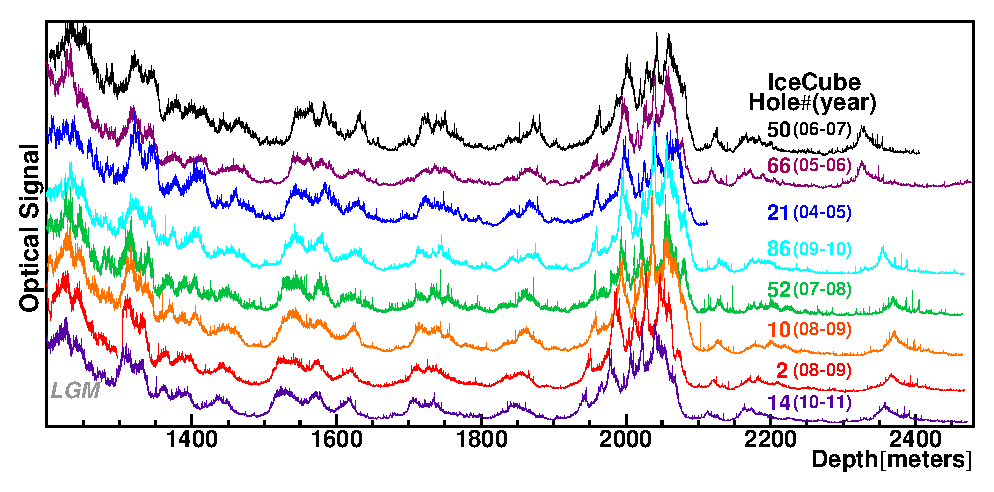
\includegraphics[width=0.9\textwidth]{dustlogger.eps} 
\caption{The data from the dust loggers deployed in various drill holes in IceCube during deployment. Data from individual holes has been offset in the y direction for clarity. Larger relative values of the "Optical Signal" represent more scattering in the ice while smaller values indicate clearer ice. The "dust layer" is visible in all drill holes around 2000 m. Deepcore DOMs are deployed below this layer. Image taken from \cite{IceCube-DustLogger-Raw}.}
\label{fig:dust_logger}
\end{figure}

Peaks are present in the dust logger data due to volcanic events in the Earth's past \cite{IceCube-DustLogger1,}.
The most significant peak, a set of features around a depth of 2000 m, form what is known as the \emph{dust layer} of IceCube, a region with significantly higher scattering and absorption properties than the surrounding ice.

To improve the modeling of the glacier, dedicated measurements have been performed using light-emitting diodes (LEDs, also known as \emph{flashers} in IceCube) onboard the DOMs \cite{IceCube-SpiceMie, Description-IceCube}.
In specialized calibration runs, the LEDs are flashed at a few Hertz for a few minutes while nearby DOMs recieve the emitted light.
Monte Carlo simulations of the flashers are used with varying ice properties in order to identify the most likely properties of the ice
Each flashing and detecting DOM pair provides a set of known times, positions, and light output in the ice, allowing for the properties of the intervening medium to be determined.

\begin{figure}[h]
\centering
    \subfloat[Absorption]{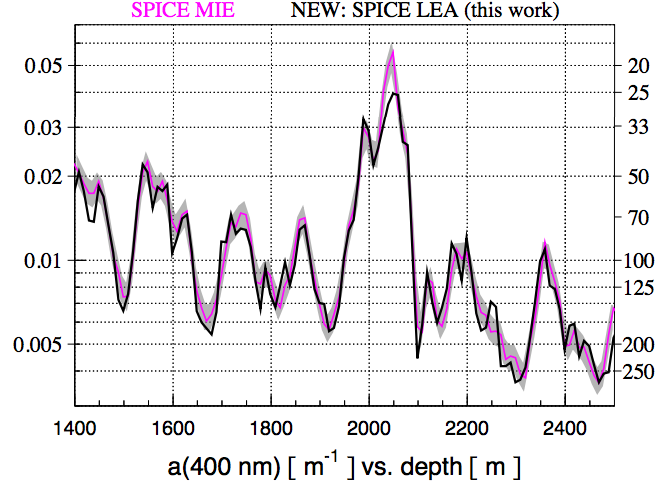
\includegraphics[width=0.4\linewidth]{absorption.png}}
    \subfloat[Scattering]{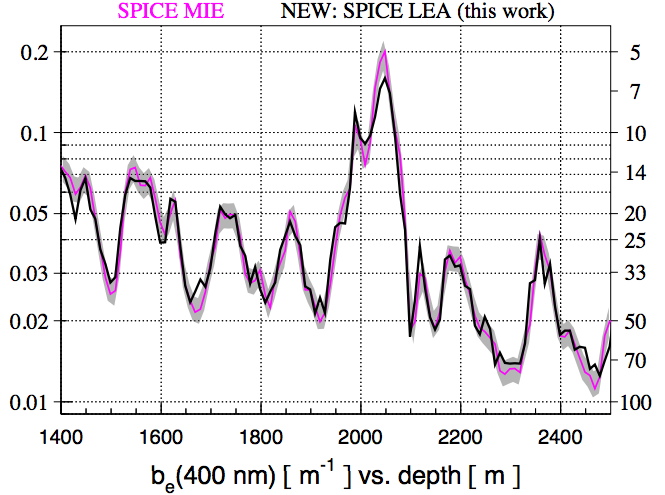
\includegraphics[width=0.4\linewidth]{scattering.png}}    
\caption{The absorption and effective scattering properties of the ice as fit to flasher data. Two models are shown representing different generations of ice models used for simulation. The "Mie" model does not include anisotropy while the "Lea" model does. Figure from \cite{IceCube-SpiceLea}.}
\label{fig:spicelea}
\end{figure}

The modern ice model used for this thesis consists of three main properties: the absorption, the scattering, and the anisotropy of the ice \cite{IceCube-SpiceLea}.
The measured properties of the absorption and scattering may be seen in Figure~\ref{fig:spicelea} while the effect of the anisotropy can be seen in Figure~\ref{fig:anisotropy}.
Scattering photons change direction, losing information about the direction of the emission source.
Absorbed photons are not visible to the detector, potentially modifying the observed number of photons and the reconstructed energy of an event.
The anisotropy, consisting of a direction and magnitude, modifies the ice properties as a function of direction due to movement and compression of the glacier over time.
The anisotropy affects both the scattering and absorption from each direction in the x-y plane and can affect the azimuthal directions of reconstructions in IceCube.

\begin{figure}[h]
\centering
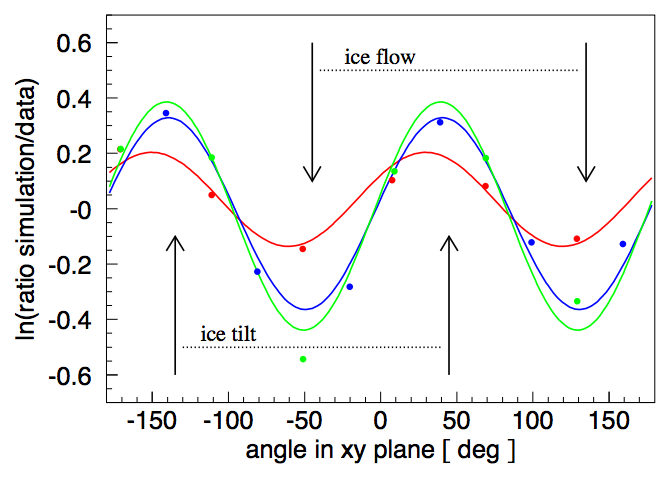
\includegraphics[width=0.6\linewidth]{anisotropy.png}
\caption{The effect of the anisotropy on the light output from a flasher on string 63. Measurements (points) are shown for receiving DOMs at three distances: at 125 m (red), at 217 m (blue), and at 250 m (green). A line is included to show the expected effect of anisotropy at each distance. The y-axis shows the ratio of a simulation of the same flasher without including anisotropy to data. A modulation is observed as a function of direction in the x-y plane.}
\label{fig:anisotropy}
\end{figure}


\label{subsec:hole_ice}
\subsection{The Hole Ice}
After the strings were deployed, each drill hole was allowed to refreeze. 
The refrozen column of ice around each string is referred to as the \emph{hole ice}.
Using a dedicated camera deployed at the bottom of string 80, the refreezing process of the hole ice has been observed over the course of several years \cite{IceCube-SwedishCamera, Description-IceCube}.
Images\improvement{find good quality swedish camera pics?} obtained from the camera show the refrozen ice divided into three distinct regions.

The outermost region, the \emph{bulk ice}, is the original glacial ice and is unaffected by the deployment of the detector.
The outer part of the drill hole shows improved clarity compared to the bulk ice.
The central region of the drill hole, a central core of about 16 cm in diameter, shows significantly worse scattering properties than the bulk ice \cite{Description-IceCube}.
This central column, referred to as the \emph{bubble column}, affects the photon acceptance of the PMT.
Measurements to characterize the hole ice are ongoing.

